% Options for packages loaded elsewhere
\PassOptionsToPackage{unicode}{hyperref}
\PassOptionsToPackage{hyphens}{url}
%
\documentclass[
]{book}
\title{Nature hacks for life}
\author{cjlortie}
\date{}

\usepackage{amsmath,amssymb}
\usepackage{lmodern}
\usepackage{iftex}
\ifPDFTeX
  \usepackage[T1]{fontenc}
  \usepackage[utf8]{inputenc}
  \usepackage{textcomp} % provide euro and other symbols
\else % if luatex or xetex
  \usepackage{unicode-math}
  \defaultfontfeatures{Scale=MatchLowercase}
  \defaultfontfeatures[\rmfamily]{Ligatures=TeX,Scale=1}
\fi
% Use upquote if available, for straight quotes in verbatim environments
\IfFileExists{upquote.sty}{\usepackage{upquote}}{}
\IfFileExists{microtype.sty}{% use microtype if available
  \usepackage[]{microtype}
  \UseMicrotypeSet[protrusion]{basicmath} % disable protrusion for tt fonts
}{}
\makeatletter
\@ifundefined{KOMAClassName}{% if non-KOMA class
  \IfFileExists{parskip.sty}{%
    \usepackage{parskip}
  }{% else
    \setlength{\parindent}{0pt}
    \setlength{\parskip}{6pt plus 2pt minus 1pt}}
}{% if KOMA class
  \KOMAoptions{parskip=half}}
\makeatother
\usepackage{xcolor}
\IfFileExists{xurl.sty}{\usepackage{xurl}}{} % add URL line breaks if available
\IfFileExists{bookmark.sty}{\usepackage{bookmark}}{\usepackage{hyperref}}
\hypersetup{
  pdftitle={Nature hacks for life},
  pdfauthor={cjlortie},
  hidelinks,
  pdfcreator={LaTeX via pandoc}}
\urlstyle{same} % disable monospaced font for URLs
\usepackage{longtable,booktabs,array}
\usepackage{calc} % for calculating minipage widths
% Correct order of tables after \paragraph or \subparagraph
\usepackage{etoolbox}
\makeatletter
\patchcmd\longtable{\par}{\if@noskipsec\mbox{}\fi\par}{}{}
\makeatother
% Allow footnotes in longtable head/foot
\IfFileExists{footnotehyper.sty}{\usepackage{footnotehyper}}{\usepackage{footnote}}
\makesavenoteenv{longtable}
\usepackage{graphicx}
\makeatletter
\def\maxwidth{\ifdim\Gin@nat@width>\linewidth\linewidth\else\Gin@nat@width\fi}
\def\maxheight{\ifdim\Gin@nat@height>\textheight\textheight\else\Gin@nat@height\fi}
\makeatother
% Scale images if necessary, so that they will not overflow the page
% margins by default, and it is still possible to overwrite the defaults
% using explicit options in \includegraphics[width, height, ...]{}
\setkeys{Gin}{width=\maxwidth,height=\maxheight,keepaspectratio}
% Set default figure placement to htbp
\makeatletter
\def\fps@figure{htbp}
\makeatother
\setlength{\emergencystretch}{3em} % prevent overfull lines
\providecommand{\tightlist}{%
  \setlength{\itemsep}{0pt}\setlength{\parskip}{0pt}}
\setcounter{secnumdepth}{5}
\usepackage{booktabs}
\ifLuaTeX
  \usepackage{selnolig}  % disable illegal ligatures
\fi
\usepackage[]{natbib}
\bibliographystyle{apalike}

\begin{document}
\maketitle

{
\setcounter{tocdepth}{1}
\tableofcontents
}
\hypertarget{sustainability}{%
\chapter{Sustainability}\label{sustainability}}


\includegraphics[width=4in,height=\textheight]{./tree.png}\\
This is the \textbf{prework} before we meet.

\hypertarget{context}{%
\subsection*{Context}\label{context}}
\addcontentsline{toc}{subsection}{Context}

\href{https://en.wikipedia.org/wiki/Nature_deficit_disorder}{Nature deficit disorder} is an experiential hypothesis for behavioral ecology. It proposes that humans spending too little time outdoors are more likely to experience behavioral challenges and reductions in cognition and mental well-being. Richard Louv first developed these ideas formally in the book entitled \href{http://richardlouv.com/books/last-child}{`Last child in the woods'} in 2008. A more recent and expansive book was published in 2012 entitled \href{http://richardlouv.com/books/nature-principle}{`The nature principle'} and another in 2019 entitled \href{http://richardlouv.com/books/}{`Our wild calling'}. These works precipitated a movement to better support programs for outdoor activities for children and stimulated incredible (but not without controversy) scientific evidence that reconnecting with nature can enhance many performance measures in people - adult and children alike. Here, we can take a sensible perspective that tracking and enhancing simple interactions in natural systems, outdoors, like provides an opportunity to explore personal performance and develop new mental and emotional skills.

There is excellent evidence in many domains of science that bridge human interaction theory with complex systems that active versus passive approaches generate different outcomes. The most effective interventions are often relatively more active, directed, and intentional depending on the field of study. Within the nature-deficit disorder framework, research that examines hands-on, active interactions with natural systems suggests that returns are significantly greater relative to passive approaches to natural systems. For instance, the Microbiome Rewilding Hypothesis (MRH) and Psycho-Evolutionary Restoration Hypothesis (PERH) suggests that nature-based health interventions that include people fixing nature (via planting, gardening, etc) generates reciprocal restoration feedbacks between the \href{https://www.liebertpub.com/doi/full/10.1089/eco.2020.0003}{people and the ecosystems}. This win-win science of reciprocity between other natural systems and the actions of people is relatively well established. This is an opportunity to be mutualistically enhance two systems in need of support - you and the natural communities we inhabit and share. A simple eudaemonic feedback loop can begin with an examination of sustainability of life choices.

\hypertarget{learning-outcomes}{%
\subsection*{Learning outcomes}\label{learning-outcomes}}
\addcontentsline{toc}{subsection}{Learning outcomes}

\begin{enumerate}
\def\labelenumi{\arabic{enumi}.}
\tightlist
\item
  Examine decisions that have impact globally.\\
\item
  Track smaller decisions that influence sustainability.\\
\item
  Explore whether changes that enhance sustainability can also promote deeper and more frequent connections with other natural systems.\\
\item
  Appreciate the limitations associated with existing and assumed norms.
\end{enumerate}

\hypertarget{schedule}{%
\subsection*{Schedule}\label{schedule}}
\addcontentsline{toc}{subsection}{Schedule}

Here is an outline of the challenges proposed to explore these principles over the course of several weeks. The first week is prework, second week is a deck and reflection on meaning and nature hacks, the third week is direct practice, and finally, the consolidation is a resolution or decision to commit some changes that are potential win-win scenarios.

\begin{tabular}{rll}
\toprule
challenge & focus & tasks\\
\midrule
1 & Explore sustainability and reciprocity with natural systems & take ecological footprint quiz, track simple life decisions, list frictions and resistance\\
2 & Nature hacks deck and discussion & reflect on meaning, list purpose, match challenges with nature\\
3 & Practice & explore nature practice, track creativity, track breath, futureproof daily practice, identify resolutions that are more significant challenges\\
\bottomrule
\end{tabular}

\hypertarget{citation}{%
\subsection*{Citation}\label{citation}}
\addcontentsline{toc}{subsection}{Citation}

Lortie, CJ (2021): Nature hacks for life. figshare. Book. \url{https://doi.org/10.6084/m9.figshare.16879312.v1}

\hypertarget{license}{%
\subsection*{License}\label{license}}
\addcontentsline{toc}{subsection}{License}

This work is licensed under a Creative Commons Attribution-NonCommercial-ShareAlike 4.0 International License.

\hypertarget{challenge-time}{%
\subsection*{Challenge time}\label{challenge-time}}
\addcontentsline{toc}{subsection}{Challenge time}

Do the \href{https://www.footprintcalculator.org/home/en}{ecological footprint quiz}.\\
Report your findings \href{https://forms.gle/s7wqpoFZh8ZJZPrz6}{here}.\\
Track frictions and points of resistance to your daily happiness and productivity.\\
Read this paper: \href{https://www.sciencedirect.com/science/article/pii/S092180091930518X?casa_token=K0Ms5gASF7YAAAAA:1NgRSJdbMDvAqIV_yEgJKoscztxm6ktNod5m_sCbSm7NZfyRMwZd9hvcqZwQzPNF-0rBDUTJGiw}{On sustainability interpretations of the Ecological Footprint.}

\hypertarget{reflection-questions}{%
\subsection*{Reflection questions}\label{reflection-questions}}
\addcontentsline{toc}{subsection}{Reflection questions}

\begin{enumerate}
\def\labelenumi{\arabic{enumi}.}
\tightlist
\item
  Did your assumptions about sustainable living reconcile with estimated global costing?\\
\item
  Are the decisions that drive footprint mostly `big' or `little' ones defined as large actions such as travel and trips or more by daily activities?\\
\item
  Did the concepts of biocapacity and ecological deficits resonante with your life decisions?\\
\item
  Are there individual or institutional-level changes that can be subtly nudged to increase capacity, capital, and resilience in sustainability?
\end{enumerate}

\hypertarget{hacks}{%
\chapter{Nature hacks}\label{hacks}}

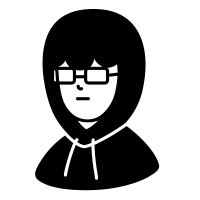
\includegraphics[width=3in,height=\textheight]{./hacker.png}

\hypertarget{context-1}{%
\subsection*{Context}\label{context-1}}
\addcontentsline{toc}{subsection}{Context}

Humans can be pretty absurd. This is not a necessarily criticism or limitation. Our capacity and desire to seek reason with meaning and suspend belief can be powerful tools for good. If we can leverage the evolutionary drives emergent from absurdity (including legacy and leisure) to promote and enable decisions that connect us with other natural systems, we benefit and those systems can be sustained. This absurdity has been captured in the hypothesis and satirical nomenclature of humans as \href{https://ojs.library.queensu.ca/index.php/IEE/article/view/13137}{Homo absurdus}. The opportunity and challenge herein is to leverage deep thinking, capacity for the abstract, and drive to create through connections with nature. Build your own new narrative. Include a nature identity, a sense of place, and active connectivity with nature. These new narratives of \href{https://www.sciencedirect.com/science/article/abs/pii/S1462901115000921}{connectivity conservation} resonate with communities provided there is an openness to observe and be mindful of the natural systems that we co-inhabit. Storytelling is a means to make science more accessible to everyone and to \href{https://www.pnas.org/content/118/15/e1914085117}{combat disinformation}. We will tell stories and use \href{https://www.jstor.org/stable/20107373?seq=1\#metadata_info_tab_contents}{narratives}, and we thus need to co-opt this cognition heuristic for leadership as individuals that decide our own lives and more widely as facilitators in organizations and teams. The scientific evidence supporting the benefits of nature connectedness through narratives in particular is \href{https://journals.sagepub.com/doi/full/10.1177/2158244019841925}{compelling} and \href{https://www.semanticscholar.org/paper/Mindfulness-and-connectedness-to-nature\%3A-A-Schutte-Malouff/8e1c1d5767b01a9f453354767168e85bd629d507}{extensive}. Natural rewards have also been proposed as major driver of \href{https://rethinkingecology.pensoft.net/article/58518/}{life advancement}.

\hypertarget{learning-outcomes-1}{%
\subsection*{Learning outcomes}\label{learning-outcomes-1}}
\addcontentsline{toc}{subsection}{Learning outcomes}

\begin{enumerate}
\def\labelenumi{\arabic{enumi}.}
\tightlist
\item
  Explore a checklist of tools or hacks from nature for performance.\\
\item
  Challenge your own absurdity and drives.\\
\item
  Develop a nature identity that includes active engagement with an outdoor pursuit or place.
\end{enumerate}

\hypertarget{challenge-time-1}{%
\subsection*{Challenge time}\label{challenge-time-1}}
\addcontentsline{toc}{subsection}{Challenge time}

\begin{enumerate}
\def\labelenumi{\arabic{enumi}.}
\tightlist
\item
  Review this \href{https://figshare.com/articles/presentation/Nature_hacks_for_life/16878808}{slide deck} and attend discussion.\\
\item
  Read \href{https://www.goodreads.com/book/show/157993.The_Little_Prince}{`The Little Prince'} short tale.\\
\item
  Read \href{https://ojs.library.queensu.ca/index.php/IEE/article/view/15122}{`The Little Prince is an ecologist'} comment paper.\\
\item
  \href{http://www.testmycreativity.com}{Test your creativity} using this short test.\\
\item
  Reflect on your scores and the radial plot and how connectedness can enhance some of the measures.
\end{enumerate}

\hypertarget{reflection-questions-1}{%
\subsection*{Reflection questions}\label{reflection-questions-1}}
\addcontentsline{toc}{subsection}{Reflection questions}

\begin{enumerate}
\def\labelenumi{\arabic{enumi}.}
\tightlist
\item
  Interactions are fundamental to all living organisms. To what extent does interaction theory, very broadly speaking, inform the ecology of your life?\\
\item
  Do you have an outdoor identity? If you could change this view, what would you innovate or augment for this self-vision? Even one mountain climbed makes you a climber. Or one bird spotted and identified a small step to becoming a birder.\\
\item
  Are there some of the nature hacks proposed (or new alternatives you envision) that can be used to restore, recharge, or rev up your creative performance and cognitive clarity?
\end{enumerate}

\hypertarget{practice}{%
\chapter{Daily practice}\label{practice}}

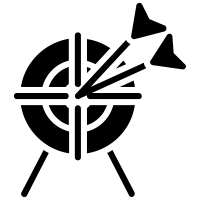
\includegraphics[width=3in,height=\textheight]{./practice.png}

\hypertarget{context-2}{%
\subsection*{Context}\label{context-2}}
\addcontentsline{toc}{subsection}{Context}

Practice makes permanent. Extensive evidence suggests that short duration, high frequency interventions in outdoor, experiential physical practice produce the most consistent and significant returns in \href{https://www.tandfonline.com/doi/full/10.1080/02640414.2020.1794763}{cognition and in health}. Here, we explore at least three of the frameworks open to innovation for boosts in performance cognitively and emotionally.

\href{https://www.nature.com/articles/s41598-019-44097-3}{Passive outdoor time} can include observation, sitting, and breath work. This category can also include taking calls outside or outdoor meetings. Nature can become the backdrop, and it is not necessarily the primary focus.

Active outdoor interactions can include observation similar to passive but directs attention to better mapping and \href{https://ellisonchair.tamu.edu/health-and-well-being-benefits-of-plants/}{identifying with natural complexity}. Typically, attention is directed to the natural systems. The natural system is the focus.

\href{https://www.tandfonline.com/doi/abs/10.1080/09603120500155963}{Green exercise} is doing a \href{https://pubmed.ncbi.nlm.nih.gov/22480735/}{short physical activity outdoors} as a mechanism to either restore or prime cognition and creativity. It can also dramatically enhance \href{https://www.mdpi.com/1660-4601/16/6/937}{emotional wellbeing}. The focus is split between interacting with the natural environment and the activity.

\hypertarget{learning-outcomes-2}{%
\subsection*{Learning outcomes}\label{learning-outcomes-2}}
\addcontentsline{toc}{subsection}{Learning outcomes}

\begin{enumerate}
\def\labelenumi{\arabic{enumi}.}
\tightlist
\item
  Explore some of the hacks \href{https://figshare.com/articles/presentation/Nature_hacks_for_life/16878808}{suggested previously} in this course of study.\\
\item
  Contrast at least three options for boosted performance from nature ninja thinking.\\
\item
  Develop a nature identity.
\end{enumerate}

\hypertarget{challenge-time-2}{%
\subsection*{Challenge time}\label{challenge-time-2}}
\addcontentsline{toc}{subsection}{Challenge time}

\begin{enumerate}
\def\labelenumi{\arabic{enumi}.}
\tightlist
\item
  Practice passive `how low can you go' outdoor time. Try for only 12mins total per day outside. Sit outside to recover, and apply a diffuse focus to natural observation.\\
\item
  Download \href{https://www.inaturalist.org}{iNaturalist app}. For one week, identify a single plant, bird, or other animal daily. Alternatively, download any \href{https://www.hortibiz.com/newsitem/news/9-best-plant-identification-app-choices-of-2020/}{nature ID app} such as \href{https://www.picturethisai.com}{PictureThis}. Do the identifications and just keep track yourself in a notebook.\\
\item
  Explore green exercise. Take a meeting outside and walk, take a call outside, walk somewhere new a few times a week, do a short run, jog for 12 mins only, or stretch outside.
\item
  Read the paper \href{https://www.fs.usda.gov/treesearch/pubs/38787}{`Understanding the transformative aspects of the Wilderness and Protected Lands experience upon human health'}. Reflect on small or large changes in how you select where you go or where you engage with natural space. It does not have to be a park or pristine protected area. It has be special only to you. There is excellent evidence that any space that you call your `own' and feel connectedness to enhances health.\\
\item
  Retake this \href{http://www.testmycreativity.com}{creativity test} or try the \href{https://www.ideo.com/blog/build-your-creative-confidence-thirty-circles-exercise}{thirty-circles test}, outside with a clipboard, and show the outcome to someone else for fun feedback.
\end{enumerate}

\hypertarget{reflection-questions-2}{%
\subsection*{Reflection questions}\label{reflection-questions-2}}
\addcontentsline{toc}{subsection}{Reflection questions}

\begin{enumerate}
\def\labelenumi{\arabic{enumi}.}
\tightlist
\item
  Was there a category of outdoor interaction that most suited your needs and was more easily reconciled with existing routines? Passive recovery time, active natural observation, or green exercise (instead of some of the time you might allocate to the gym or other workout times).\\
\item
  Did an identity such as birder, walker, open-air thinker, outdoor meeting person, plant lover, or outdoor reflection seem like a good fit?\\
\item
  What impediments or frictions long-term will present challenges to nature ninja hacks - at the fine-grain resolution of daily experiential boosts?\\
\item
  Given the evidence presented previously for reciprocal restoration benefits and feedback loops between people and natural systems when we `fix up' nature, how can you consider taking outdoor experiential interactions to this next level? This would not be at at the daily level but instead include monthly park or beach cleanups, native planting, weed removal, tending your plants indoors or outdoors weekly, or other processes that demonstrate and affirm benefits to both systems - you and the other natural systems.
\end{enumerate}

  \bibliography{book.bib,packages.bib}

\end{document}
